\documentclass[lettersize,journal]{IEEEtran}
\usepackage{amsmath,amsfonts}
\usepackage{algorithmic}
\usepackage{array}
\usepackage[caption=false,font=normalsize,labelfont=sf,textfont=sf]{subfig}
\usepackage{textcomp}
\usepackage{stfloats}
\usepackage{url}
\usepackage{verbatim}
\usepackage{graphicx}
\usepackage{amsfonts}
\usepackage{amsmath}
\usepackage{amssymb}
\usepackage{amsthm}
\usepackage{pdfpages}
\usepackage{amssymb}
\usepackage{listings}
\usepackage{proof}
\usepackage{xcolor}
\usepackage{titlesec}
\usepackage{rotating}
\usepackage{float}
\usepackage{tikz}
\hyphenation{op-tical net-works semi-conduc-tor IEEE-Xplore}
\def\BibTeX{{\rm B\kern-.05em{\sc i\kern-.025em b}\kern-.08em
    T\kern-.1667em\lower.7ex\hbox{E}\kern-.125emX}}
\usepackage{balance}

\definecolor{OliveGreen}{rgb}{0,0.6,0}
\lstset{
  language=C,
  frame=tb,
  aboveskip=3mm,
  basicstyle=\footnotesize\ttfamily,
  numbers=left,
  stepnumber=1,
  numbersep=10pt,
  tabsize=4,
  columns=flexible,
  numbers=none,
  numberstyle=\tiny\color{gray},
  keywordstyle=\color{blue},
  commentstyle = \color{OliveGreen},
  stringstyle=\color{purple},
  breaklines=true,
  breakatwhitespace=true,
  showstringspaces=false,
  tabsize=3,
}

\begin{document}
\title{JavaScript Framework for Actor-Based Programming Review Report}
\author{Andrew Buhagiar}

\maketitle

\begin{abstract}
This dissertation explores the suitability of the actor model when used to bring concurrency and parallelism to JavaScript. Actors are concurrent isolated units of computation which process messages using their predefined behaviour. The prototype takes the form of two frameworks for both the Node.js and browser environments respectively, allowing developers to intuitively reason about engineering JavaScript programs through the spawning and sending of messages to actors.

Isolated actors can be safely spawned on remote devices over a network as well as utilise multiple cores on a local processor. This allows for distributed and parallel computation which have the potential of shortening the time taken when executing computationally intensive tasks. A WebSocket server is used to connect a finite number of Node.js instances and browsers hosting actors over the network. Faster communication links are explored using inter-process communication when hosting multiple processes on a local device. The prototype abstracts the adaptive use of different communication links and provides location transparency for remote actors.

Benchmarks analyse the frameworks' performance when used on a single instance using Node.js or a browser, as well as the speedup introduced when utilising additional local or distributed cores working on the same task. This dissertation's implementation is evaluated against existing JVM and JavaScript actor framework implementations. It performs Savina benchmarks faster than other actor frameworks while demonstrating near linear performance when distributing a task over multiple cores. The relative performance of the communication links used when distributing actors is also explored.
\end{abstract}

\begin{IEEEkeywords}
Concurrency, Parallelism, Web Development, IoT
\end{IEEEkeywords}

\section{Introduction}
The JavaScript programming language~\cite{ecmascript} is widely used for client applications on the browser and benefits from a growing popularity of server-side applications using environments such as Node.js~\cite{nodejs}. It is a single-threaded language which lacks an intuitive way to program in a parallel and distributed fashion. 

This dissertation presents a prototype which enables developers to build actor-based~\cite{hewitt1973session, 43years} systems in JavaScript. Developers can use actors as concurrent units of computation which can be deployed either locally or remotely on multiple Node.js runtimes and browsers. This allows developers to intuitively distribute work amongst multiple processors and devices to fully utilise the hardware available in servers and modern computers.

%Why Actors
Actors communicate with each other using messages, which are stored in the receiving actor's message queue. A message is processed by executing the predefined actor behaviour. The actor model is a good fit for JavaScript's event loop~\cite{eventloopbrowser, eventloopnode} as they are both event-driven, and the model has already achieved success in the telecommunications industry~\cite{erlang}. It has also been recently used for implementing distributed systems in languages such as Erlang and Scala/Akka~\cite{haller2012integration}.

%The Frameworks
The developed prototype takes the form of two frameworks for the browser and Node.js environments respectively. The frameworks' interoperable API abstracts the prototype's internal mechanisms which spawn and interact with actors, allowing developers to intuitively make use of the actor model in their code.
\section{Objectives}
This dissertation will explore how to design and implement actor frameworks for the JavaScript language. The frameworks' suitability will be assessed on the basis of performance, scalibility, and intuitiveness of use. The objectives of the study are as follows:
\begin{enumerate}
    \item Allow developers to easily define and spawn actors through the framework API on Node.js or a browser. Actors should be able to send messages to each other as well as spawn more actors. Full interoperability should be provided when using the framework across the two environments.
    \item Allow developers to spawn and interact with actors residing in different Node.js and browser instances through different network links. Node.js Cluster~\cite{cluster} can be used for IPC between node processes, while Web Workers~\cite{webworkers} can be used for communication between the primary thread and its spawned workers. When such communication links are not available, the network stack is involved by using WebSockets~\cite{websocket} for flexible communication to link remote processes and devices.
    \item Provide location transparency when dealing with actor references. Interacting with a local actor should be the same as interacting with a remote actor when using the API.
    \item Benchmark the performance and scalability of the developed prototype as well as assess its feasiblity for adoption by developers.
\end{enumerate}
\section{Literature Review}
\subsection{Concurrency and Parallelism on JavaScript}
JavaScript is an implementation of the ECMAScript~\cite{ecmascript} design. The ECMA-262 language has multiple published editions, each of which serves as a blueprint for JavaScript's next stable release. JavaScript relies on a single-threaded non-blocking event loop~\cite{eventloopbrowser, eventloopnode} which does not support parallelism, raising an issue when high performance computing~\cite{highperformance} is required. Browser Web Workers~\cite{webworkers} and Node.js child processes~\cite{nodejs, cluster} can be used to bring parallel computation to JavaScript~\cite{concurrencyjs, spidersjs}.

A system achieves concurrency when multiple tasks or processes can progress at the same time~\cite{concurrency}. The sub processes communicate with each other to solve a particular task, without requiring knowledge of the full system implementation. Using JavaScript Promises~\cite{promises}, developers can manage the data returned by concurrently running asynchronous operations. JavaScript later developed the async/await syntax~\cite{async} where async functions always return a Promise resolving into the value that is returned by the function. An await expression suspends the execution of an async function until the Promise can be consumed, eliminating the need to define Promise chains. ECMAScript also provides the SharedArrayBuffer~\cite{sharedarraybuffer} constructor for shared-variable concurrency. Memory can be shared across agents in different Cluster processes or Web Workers.

\subsection{The History of the Actor Model}
The actor model was first introduced by Carl Hewitt~\cite{hewitt1973session, 43years} in 1973 for research in artificial intelligence. It defines actors as computational agents which execute a uniform behaviour when they receive a message. Hewitt argued that the actor metaphor can be applied to processes and daemons amongst other things. Two years later, Carl Hewitt supported in writing a draft of PLASMA~\cite{plasma, chewitthowto}, the first actor language. In this language, actors communicate with each other using messages, while the receiver processes the received messages using its pre-defined computation. Based on the message's contents, the actor may choose one of the different behaviours which may involve sending messages to other actors.

The actor model was clarified by Gul Agha~\cite{agha1985actors} in a paper published in 1986. While Carl Hewitt's paper set the foundation of the potential applications of the actor metaphor, this paper focuses on how actors can be used to create expressive, simple, and intuitive programming languages. It identifies actors as computational agents which map incoming messages to a behaviour. Such behaviour may include communicating with other actors, deciding how the next incoming communication will be processed as well as creating more actors. Actors benefit from asynchronous communication when sending messages as it allows each actor to communicate with itself without waiting, increasing overall efficiency. The paper recognises that the delivery of messages is not guaranteed on a network, and that all receiving buffers are bounded.

Nowadays, several variants of the actor model are used to fit the requirements of modern languages and frameworks. Popular languages such as Scala~\cite{scala} with Akka~\cite{akka} and Elixir~\cite{elixir} (built on top of Erlang~\cite{erlang}) use the actor model to build scalable distributed systems.

\subsection{Similar Work}
Several JavaScript frameworks which implement the actor model are available on the node package manager (npm) and in public git repositories. They exhibit a variety of designs, each with their own strengths and weaknesses, which will be explored in the remainder of this section.

\textbf{Nact}~\cite{nact} allows developers to spawn an actor by first defining the actor's behaviour through a function with the state, message, and system context as the parameters. The function is called for every message that is processed by the spawned actor. The framework does not have inbuilt functionality to communicate with actors over the web, as it makes use of a JavaScript REST API to expose actors to the web in one of the provided examples.

\textbf{Spiders.js}~\cite{spidersjs} identifies the problem of different APIs being used for Web Workers and child processes, both of which are inspired by the actor model for constructing parallel systems using JavaScript. This project focuses on defining a single actor model API, no matter if it is a client or server-side application. This framework allows for communication with actors over a network when provided with the machine's IP address and port number it is listening on. Spiders.js spawns a new Node.js child process or Web Worker for each actor to provide each actor with its own thread of control, allowing developers to engineer systems using Communicating Event Loops (CEL).

\textbf{TigerQuoll}~\cite{tigerquoll} takes a different approach when providing parallelism to the language. The paper states that the actor model is too limited for the requirements of more complex patterns that occur in modern applications. Instead, it allows developers to use regular event-based programming to register events for parallel processing. 

\textbf{Kurt Micallef}'s paper~\cite{kurt} also brings parallelism to JavaScript by exploiting ES6 Generators and several web technologies. His prototype allows for developers to engineer parallel and distributed programs over both browsers and Node.js, provided that development is done through the use of Communicating Sequential Processes (CSP).
\section{Design and Implementation}
Through the fulfillment of this dissertation's objectives, developers are able to spawn actors on both Node.js and browser instances. Furthermore, actors can communicate with each other to collaboratively process tasks in a distributed environment. The prototype's design must be faithful to the actor model theory while taking advantage of the JavaScript runtime, both of which were discussed in the previous chapter. Ideally, the prototype should be feasible to adopt by developers and demonstrate a low overhead over utilising plain JavaScript.

\subsection{Actors on a Single Node.js or Browser Instance}
\subsubsection{Actor Design}
Gul Agha's paper~\cite{agha1985actors} prompts the API to allow for the creation of actors and the ability to send communications to the spawned actors. Communications sent to actors take the form of JavaScript objects due to their structural flexibility and conformity with Gul Agha's definition of a “tuple of values”. Actors are defined to have history sensitivity, which prompts each actor to hold a local isolated state, which also takes the form of a JavaScript object. The actor's behaviour takes the form of a conventional JavaScript callback function, which has the actor's state, message, and self address as function parameters. Since JavaScript provides first class functions, the behaviour definition is stored and called when required.

The API returns an actor reference when one is spawned, which can then be fed into the send function as a parameter. The actor behaviour is invoked when processing each received message, and may manipulate the actor's state which is initially defined through a parameter passed into the spawn function. The actor behaviour may also use the API to spawn and communicate with other actors. Finally, a function to terminate an actor is provided, with the option for whether it should process its remaining messages. This function takes in an actor reference similar to the send function. The following code is a TypeScript~\cite{typescript} definition of the API design so far.
\begin{lstlisting}
interface ActorBehaviour {
    (state: object, message: object, self: ActorReference): void
}
spawn = (initialState: object, behaviour: ActorBehaviour): ActorReference
send = (actor: ActorReference, message: object): void    
terminate = (actor: ActorReference, force: boolean)
\end{lstlisting}

\begin{figure}[H]
    \begin{centering}
        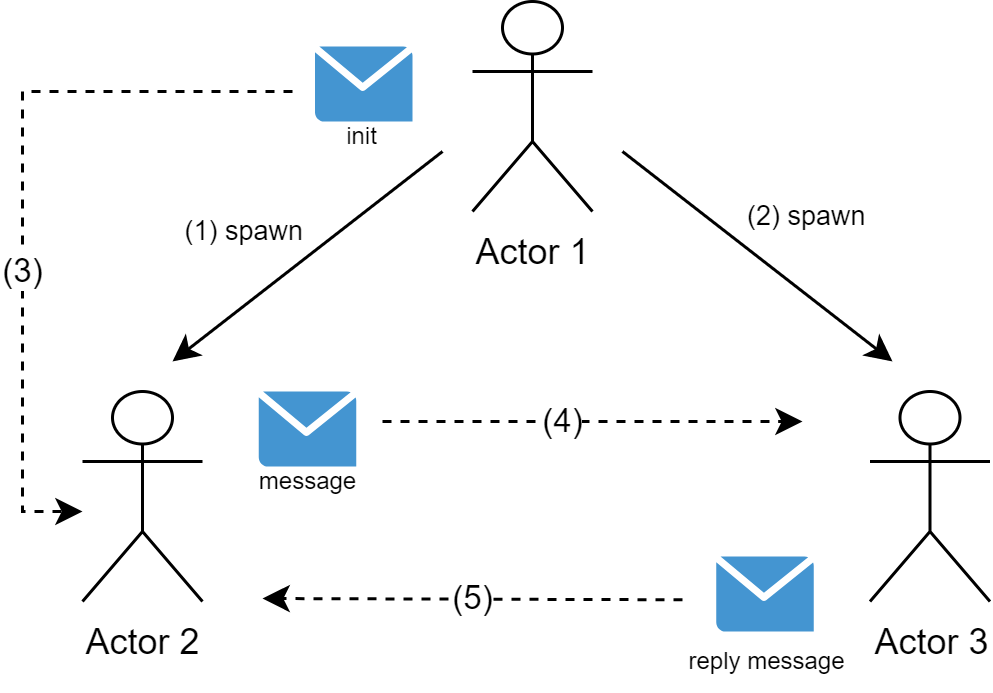
\includegraphics[width=230px]{resources/actors.png}
        \caption{Spawning Actors and Sending Messages}\label{fig:actors}
    \end{centering}
\end{figure}
\subsubsection{Actor Anatomy}
The internal composition of an actor inside the framework is at the heart of the API's features. An actor takes the form of an object which contains its maintained state as well as its behaviour as an executable function. Each actor stores a name so that it can be uniquely identified in a local instance, and a `node' number which allows other clients to uniquely identify the actor's network location. Whether the actor processes incoming messages is also stored. The TypeScript interface below defines what an actor is composed of.
\begin{lstlisting}
//TypeScript object interface for an Actor
interface Actor {
    name: string,                       
    node: number,                       
    state: { [key: string]: any },      
    behaviour: ActorCallback,           
    active: boolean                     
}
\end{lstlisting}
\subsubsection{Actor Runtime}
The JavaScript event loop~\cite{eventloopbrowser, eventloopnode} is responsible for executing the application code. The language's runtime has an event queue where each event is mapped to a function which processes that event. The event loop waits for the arrival of an event and processes the queue of events when there is a backlog in the event queue. Each event is processed to completion before other events are processed. The actor model also maps received messages onto functions, which act as message handlers. Therefore, the prototype's implementation takes advantage of the similar philosophies between the JavaScript runtime and the actor model.

The implementation acts as a wrapper of the JavaScript event loop. Once a message is received by an actor, it schedules the processing of the message on the JavaScript event loop. This is done by scheduling a microtask~\cite{microtasks}, which is an event queued to execute before the start of the next iteration of the event loop. The microtask is scheduled by creating a Promise which is immediately resolved. This behaviour is similar to using Node.js' \textbf{process.nextTick()}~\cite{nexttick}, which is more efficient than using the JavaScript's \textbf{setTimeout()} function, as it would otherwise schedule a macrotask which executes in the following iteration of the event loop.
\begin{lstlisting}
//Code which schedules the processing of a received message
Promise.resolve().then(() => {
    if (message !== undefined && localActor.active)
        localActor.behaviour(localActor.state, message, { name: localActor.name, node: localActor.node });
})
\end{lstlisting}
JavaScript only has one microtask event queue, so the order in which messages are sent matches the order in which they are processed by the set of receiving actors. JavaScript also processes each microtask to completion before processing the next, thus ensuring that at most one actor is processing a message at any point in time on a single Node.js or browser instance.
\subsection{Actors on Multiple Node.js or Browser Instances}
\subsubsection{Actors on a Distributed Network}
The developer should be able to spawn actors remotely on a distributed network. A peer-to-peer system is first considered to connect nodes which host actors. Each peer would have a list of nodes to establish connection with. While this would eliminate the additional network hop introduced by an intermediate server, the number of connections performed would be $n!$ if each node is listening for connections and connects to every other node. Furthermore, manually entering which peers each node needs to establish connection with is tedious. Instead, the prototype opts for a central WebSocket server for distributed networking, as each node can communicate with the rest of the network using only $n$ connections.

The WebSocket server expects a fixed number of $n$ connected clients before it starts accepting communication to be forwarded between nodes. The server logic was developed separate from the actor framework, and assumes that connections are not terminated in the duration of its runtime. The WebSocket server assigns a unique identifier to each connected client which is broadcasted when the server establishes the expected number of connections. This allows developers to uniquely identify clients on the WebSocket network.

This mode of establishing communication between nodes has several advantages and disadvantages. The centralised WebSocket server effectively creates a barrier, which lifts when the expected number of clients are connected and can communicate with each other. Once the number of expected clients connect, each client is granted communication with the entire network at the cost of the network hop over the WebSocket server. The centralised server also simplifies the logic of uniquely identifying each connected client, which is a simple iterative naming scheme in the order in which clients connect. Connecting to the server should take the form of an API function call which returns a Promise. This Promise resolves when the server broadcasts to the client that it is ready to forward information to the other connected clients.
\begin{lstlisting}
init = (url: string, timeout:number): Promise<object>
\end{lstlisting}

\subsubsection{Remote Spawning Mechanism}
The developer must be able to refer to actors which exist in remote nodes. API functionality to remotely spawn actors on other nodes would address this requirement as it would allow for one instance to get references to actors it remotely spawned. Security is potentially an issue since actors could be spawned remotely on machines by malicious peers. However, it allows for expressive programs which can centrally load balance work on a distributed network by sending messages to the remote actors using the obtained references through remote spawning.
\begin{lstlisting}
spawnRemote = (node: number, state: object, behaviour: ActorBehaviour, timeout: number): Promise<ActorReference>
\end{lstlisting}

The \textbf{spawnRemote} function sends a request to spawn an actor to the remote node. The request has embedded within it the string representation of the actor behaviour, which is reconstructed as a function on the recipient end. On the recipient's side, the client spawns an actor with the sent behaviour and initial state. It locally generates the spawned actor's name and embeds it in an acknowledgement sent to the remote spawner. Once this acknowledgement is received by the spawner, it constructs the actor reference using the received actor name, and resolves the Promise.

\subsubsection{Local Parallelism on Multicores}
The WebSocket server provides distribution for any Node.js or browser client wishing to communicate with actors hosted on other connected clients. However, a developer might want to host multiple instances on a local multicore device to make up for JavaScript's single-threaded runtime when distributing actors. The WebSocket server requires an intermediary network hop as well as the network layer, both of which can be avoided by using Node.js Cluster~\cite{nodejs, cluster} and browser Web Workers~\cite{webworkers}. These methods rely on inter-process communication (IPC), which allows direct communication between the spawner and the workers over shared memory. Each of the spawned workers can also be treated as separate instances when connected to the WebSocket server for communication with remote devices.

This would require changing the API's \textbf{init} function to allow the developer to specify the number of additional workers to spawn and connect to the WebSocket server, resulting in the function definition below. The default number of workers is set to 0, where the instance would not spawn any workers.
\begin{lstlisting}
init = (url: string, timeout: number, numWorkers: number = 0): Promise<object>
\end{lstlisting}

\subsection{Location Transparency}
Location transparency entails that the developer does not need to specify whether the actor resides in a spawned Web Worker or Node.js child process, as well as whether it is a local or remote actor. This is done by embedding the assigned network number as well as the actor's unique name inside the actor reference returned by the API's spawning functions.

Using the returned ActorReference object from the \textbf{spawn} or \textbf{spawnRemote} function, an actor can be uniquely identified across the network. The developer can pass the actor reference as a parameter to the \textbf{send} function to send that actor a message. Internally, the framework looks at the actor reference's network number and chooses the fastest available link.

The convenience of location transparency is provided through the WebSocket server, which provides unique names to each of the connected clients. Actors on different clients in the network communicate with each other through the WebSocket server, which routes each of the messages accordingly. This comes at the cost of having each of the distributed nodes relying on a potentially failing central point.
\section{Evaluation}
Savina~\cite{savina} is a benchmark suite defined for actor-based systems which is implemented using this disseration's framework. These benchmarks are explained and discussed in the FYP report alongside other benchmarks which are not mentioned in this document. Unless otherwise stated, the following hardware and software was used to run the benchmarks.
\begin{itemize}
    \item OS --- Ubuntu 20.04 focal (64 bit)
    \item CPU --- Intel Core i7--1065G7. 4 cores at 3.9GHz with hyper-threading disabled
    \item RAM --- LPDDR4 16GB (2$\times$8GB) at 4267MHz
    \item Node.js --- v16.14.0
    \item Google Chrome --- v100.0.4896.88 (Official Build)
\end{itemize}

\subsection{Micro-Benchmark Performance}
The Savina benchmark suite defines micro-benchmarks which test specific actor runtime features. Figure~\ref{fig:micro} compares the execution times between the browser and Node.js implementations of Savina's micro-benchmarks. In general the Node.js and browser implementations for the actor framework have consistent and similar results. However, Node.js performs worse when a large number of messages are on the event queue.
\begin{figure}[H]
    \begin{centering}
        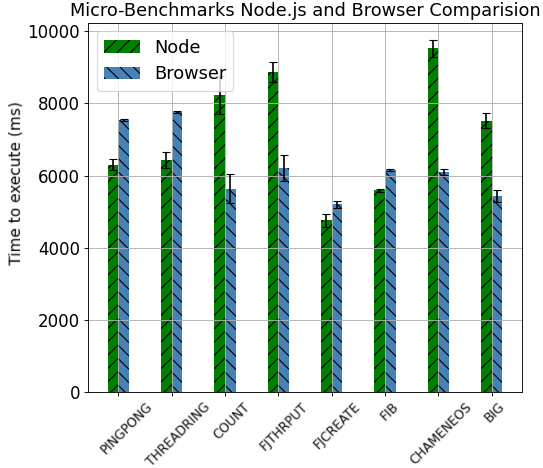
\includegraphics[width=230px]{resources/micro.png}
        \caption{Node.js and Browser Comparison for Micro-Benchmarks}\label{fig:micro}
    \end{centering}
\end{figure}

\subsection{Shared Memory Performance}
The Savina benchmark suite defines parallel benchmarks where multiple actors perform computation in parallel to complete a task. Each of the explored parallel benchmarks in the dissertation benefit from master-worker parallelism, where a master actor farms tasks to worker actors which will start execution in parallel. Then, the workers report their results to the master, which aggregates the collected data, producing the final result. The framework is tested by first executing the benchmark using only one master and one worker in separate runtimes, where the worker is limited by JavaScript's single-threaded nature.  Next, two workers are spawned on separate runtimes, each of which is ideally assigned half of the computational load by the master. Since the framework is tested on a system which houses four cores, the benchmarks are scaled up to four worker runtimes running in parallel. The speedup introduced over running on one worker is tested and plotted in the figure below, where near linear results can be observed.
\begin{figure}[H]
    \begin{centering}
        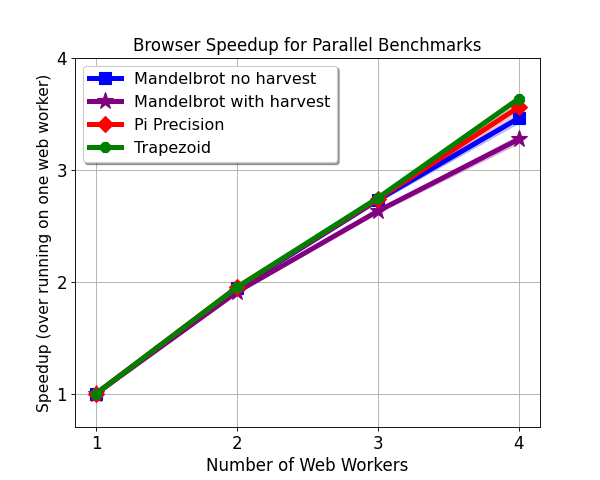
\includegraphics[width=250px]{resources/browser_speedup.png}
        \caption{Browser Shared Memory Speedup}
    \end{centering}
\end{figure}
\subsection{Distributed Memory Performance}
The following benchmark experiments with having actors hosted across distributed memories collaborating in rendering an image of the Mandelbrot set~\cite{mandelbrot} without harvesting. A Raspberry Pi 4 is used to host a WebSocket server, which handles the forwarding of messages between the connected devices. The diagram below shows the speedup introduced when connecting a new device on the network with the following specifications.
\begin{itemize}
    \item OS --- Windows 10 Home (64 bit)
    \item CPU --- Intel Core i5--10500 6 cores up to 3.10GHz with hyper-threading enabled
    \item RAM --- DDR4 32GB (4$\times$8GB) at 2666MHz
\end{itemize}
In addition to the four workers and master hosted on the four-core device, new workers are incrementally added and connected to the WebSocket server on the new device. While avoiding data harvesting to minimise the network dependency, one can observe a consistent speedup when adding more workers on the second device, with Node.js achieving slightly better speedup with a larger number of workers. Despite network overhead being introduced when distributing actors over the network, the second device makes up for this with its faster processing time.
\begin{figure}[H]
    \begin{centering}
        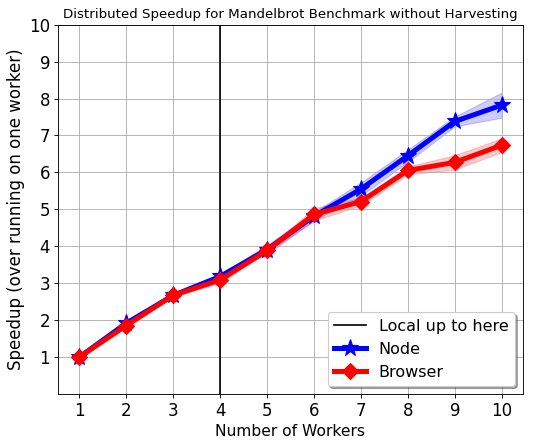
\includegraphics[width=230px]{resources/distributed_memory_speedup.png}
        \caption{Node.js and Browser Comparison for Distributed Memory Speedup}
    \end{centering}
\end{figure}
\subsection{Single Instance Actor Based System Case Study}
When making use of actors in a single instance, the developer is required to make use of three API functions taking in two parameters each. These functions allow the developer to \textbf{spawn} actors, \textbf{send} messages to them, and \textbf{terminate} them to free up memory. The example below makes use of these three API functions to build two communicating actors which send messages to each other. The first actor outputs the values 5, 3 and 1, while the second actor outputs the values 4 and 2, as they send each other decrementing values until both terminate when receiving a value of 0 or less.
\begin{lstlisting}    
import actors from 'actors.js';
const {spawn, terminate, send} = actors

const pingPongBehaviour = (state, message, self) => {
    send(message.replyTo, {val: message.val-1, replyTo: self});
    if(message.val-1 < 0)
        terminate(self)
    else    
        console.log(message.val);
};

const pingActorRef = spawn({}, pingPongBehaviour);
const pongActorRef = spawn({}, pingPongBehaviour);
send(pingActorRef, {replyTo: pongActorRef, val: 5});
\end{lstlisting}
\section{Conclusions}
The prototype successfully provides an intuitive, scalable, and fairly performant JavaScript implementation of the actor model for both the Node.js and browser environments. The functionality is exposed through an API as a collection of functions which abstract the concept of actors as well as the use of numerous communication links for distributed and parallel programming. The developed framework exploits the similarities between Gul Agha's~\cite{agha1985actors} definition of the actor model and JavaScript's event loop~\cite{eventloopbrowser, eventloopnode} to minimise the slowdown introduced when utilising the framework. 

Each of the dissertation's four objectives were fully achieved. The two frameworks allow developers to spawn and send messages to actors on local Node.js and browser instances respectively. Messages are processed through the execution of the predefined behaviour of actors (Objective 1). Using several web technologies, developers are not limited to a single instance when spawning actors, as they can spawn actors on remote browsers and Node.js instances (Objective 2). Once actors are spawned either locally or remotely, the framework internally handles local and remote communication without additional input required by the user (Objective 3, location transparency).

The framework was evaluated using both qualitative and quantitative analysis (Objective 4). Quantitative benchmarks yielded sane results when using the Savina actor benchmark suite~\cite{savina}. The separate Node.js and browser frameworks demonstrated similar performance in most cases, with reasonable standard error. The speedup of parallel actors was observed to be close to the ideal linear speedup when utilising up to four cores, and achieved a reasonable speedup when distributed actors were introduced. 

The developed actor framework is not without its limitations. Distributed clients must connect to a provided WebSocket server to communicate with their peers. Each client must wait for the expected number of clients to connect before being allowed to communicate with each other, and communication over the server introduces an intermediary network hop. The distribution of actors could be done using peer-to-peer WebSocket connections at the cost of more complex synchronisation and requiring each client to listen for connections.
\bibliographystyle{ieeetr}
\bibliography{references}
\end{document}


